\documentclass[sigconf,natbib=true,anonymous]{acmart}
%% WSDM 2027 — 0822 layout/LOVO/Fig.1 pass (old live file: main_wsdm2027_v3.tex)
%% Main-table GTS-Last/Random: cutoff-fit, no-cross (Beauty wrap_beauty_*; Toys/Grocery wrap_*).
%% tab:early: matched-protocol Early v2 (2026-08-19): cutoff-fit, no-cross, [0.6,0.1,0.1].
%% tab:lovo: GTS-Last warm, wrap_*_mv, 3-seed mean (2026-08-19).
%% 0820: variants renamed TF / TF+LLM / TF+MV (TF-anchored); tab:shift/tab:bucket =
%%       all-target catalog-level context (not a direct explanation of warm MRR);
%%       hybrid results written in (hybrid_ts_gts_last.csv + random seeds);
%%       cohort counts in 3.1; UniSRec described as adapted backbone; roy2007effective added.
%% 0822: LOOV→LOVO; drop repeated Early-window sentence; RQ heading kept with list;
%%       Fig.1 annotation moved out of bars, mathtext ≈.
%% 0823: WORKING de-AI-tone pass on top of 0822.
%% Pass 1: RQ1 LOO / Last-Random / hybrid hedge trims.
%% Pass 2: Intro widely-held/seldom-examined; LOO ``not merely''; Implications
%%         narrow-vs-broad restatement; practitioner-4 sermon; conclusion
%%         template lead + community-should closer; ethical restack.

\settopmatter{printacmref=false}
\renewcommand\footnotetextcopyrightpermission[1]{}
\setcopyright{none}
\acmConference[WSDM'27]{Proceedings of the 20th ACM International Conference on Web Search and Data Mining}{February 15--19, 2027}{Hong Kong}
\acmYear{2027}
\acmDOI{}
\acmISBN{}

\usepackage{booktabs}
\usepackage{multirow}
\usepackage{amsmath}
\let\Bbbk\relax
\usepackage{amssymb}
\usepackage{graphicx}
\usepackage{subcaption}
\usepackage{siunitx}
\usepackage{xspace}
\usepackage{enumitem}
\usepackage{microtype}
\usepackage{balance}
\usepackage{placeins}
\usepackage{float}
\usepackage{hyperref}
%% Do not hyphenate short function words; prefer geo-metric / sin-gular over geomet-ric / singu-lar.
\hyphenation{under measure geo-metric sin-gular}

\newcommand{\tfidf}{\textsc{TF-IDF}\xspace}
\newcommand{\llm}{\textsc{LLM}\xspace}
\newcommand{\tfllm}{\textsc{TF+LLM}\xspace}
\newcommand{\tfmv}{\textsc{TF+MV}\xspace}
\newcommand{\base}{\textsc{SASRec}\xspace}

\begin{document}

\emergencystretch=1.2em

\title{Do More Text Views Help?\\
A Leakage-Aware Evaluation of Text Representations\\
for Sequential Recommendation}

\author{Anonymous Author(s)}
\affiliation{%
  \institution{Anonymous Institution}
  \country{}}
\renewcommand{\shortauthors}{Anonymous}

%==============================================================================
\begin{abstract}
%==============================================================================
%% Abstract claims locked to the submitted text; only variant names unified to TF / TF+LLM / TF+MV.
Text features are widely used to enrich sequential recommenders, but comparisons of lexical \tfidf against TF-anchored LLM augmentations (single-view \tfllm or multi-prompt \tfmv) are often conducted under evaluation protocols that permit temporal overlap.
We conduct a leakage-aware controlled study of ID-only, cutoff-fit \tfidf, \tfllm (a single Qwen2.5-7B view added to the \tfidf base), and \tfmv (four prompt views added to the \tfidf base) under full-ranking global temporal splitting (GTS) on three Amazon datasets, using GTS-Last as the primary protocol, GTS-Random as a robustness check, and per-user leave-one-out (LOO) as a contrast.
Three findings emerge.
First, evaluation protocol changes conclusions: across the evaluated settings, text consistently improves over ID-only on warm targets, but the relative ordering of \tfidf, \tfllm, and \tfmv changes across Last, Random, and LOO, even when Last and Random evaluate the same trained checkpoints.
Second, in a temporal-window experiment, no text representation is robustly dominant: shifting the evaluation window earlier reduces absolute performance while preserving near-ties among text variants.
Third, additional prompt views provide limited marginal value because they are highly redundant: inter-view CKA reaches $0.82$--$0.94$, the concatenated representation uses only $53$--$55\%$ of its nominal effective rank, and leave-one-view-out has negligible downstream effect.
In contrast, TF-IDF is geometrically distinct from LLM views (CKA $0.18$--$0.20$), suggesting a potentially complementary lexical--semantic axis that is not captured by adding more prompt views.
These results suggest that evaluation protocol and representation redundancy should be diagnosed before attributing gains to increasingly complex LLM text pipelines.
\end{abstract}

\begin{CCSXML}
<ccs2012>
 <concept>
  <concept_id>10002951.10003317.10003347.10003350</concept_id>
  <concept_desc>Information systems~Recommender systems</concept_desc>
  <concept_significance>500</concept_significance>
 </concept>
 <concept>
  <concept_id>10002951.10003317.10003318.10003319</concept_id>
  <concept_desc>Information systems~Content ranking</concept_desc>
  <concept_significance>300</concept_significance>
 </concept>
</ccs2012>
\end{CCSXML}
\ccsdesc[500]{Information systems~Recommender systems}
\ccsdesc[300]{Information systems~Content ranking}

\keywords{Sequential Recommendation, Text Features, Temporal Evaluation, Multi-View Redundancy, Leakage-Aware Protocol}

\maketitle

%==============================================================================
\section{Introduction}
\label{sec:intro}
%==============================================================================

Sequential recommendation predicts a user's next item from historical interactions~\cite{kang2018sasrec,sun2019bert4rec,hidasi2016gru4rec}.
Item text---titles and descriptions---is a standard way to enrich sequential recommenders and enable cross-domain transfer~\cite{hou2022unisrec,li2023recformer}.
A natural working hypothesis is that \emph{richer text always helps}: pretrained language embeddings should beat \tfidf, and multiple prompt-based views of the same item should beat a single view.
Recent work shows that pretrained language representations can improve text-enhanced sequential recommendation and transferability~\cite{hou2022unisrec,li2023recformer}, and that feature-level attention can exploit item attributes~\cite{zhang2019fdsa}.
We ask whether multiple prompt-conditioned views of the same item text---in this study, description, function, audience, and style---add complementary signal beyond a single view.
That comparison, and whether cutoff-fit \tfidf already suffices, depends on how evaluation is set up.

This hypothesis rests on fragile evaluation foundations.
Most text-enhanced sequential recommenders are validated with leave-one-out (LOO) splits that, as shown by \citet{ji2023evaluation} and \citet{sun2023reevaluation}, allow temporal overlap between training and test, making the impact on absolute metrics unpredictable and potentially distorting model comparisons.
In a deployment scenario, a recommender must predict items that a user will interact with \emph{in the future}, not reconstruct a randomly held-out historical interaction.
Global temporal split (GTS) better simulates this deployment constraint, but introduces additional design choices: the \emph{target-selection mode} (Last, Random, Successive, or All interactions per user in the test window) itself changes effective task difficulty and can alter model rankings~\cite{gusak2025time}.
Prior work has studied split effects in general~\cite{meng2020temporal,ji2023evaluation}; we show that these effects are \emph{specifically decisive} for the \tfidf vs.\ \tfllm vs.\ \tfmv comparison.

Text features also require preprocessing---vocabulary construction, IDF weighting, SVD projection, and LLM embedding whit\-ening---each of which must respect the temporal boundary.
If these statistics are computed on the full item set (including future items), the resulting features carry information unavailable at training time, introducing a form of leakage orthogonal to the train/test split itself.
We therefore enforce strict \emph{cutoff-fit} controls throughout: all text preprocessing is fit only on items appearing before the training cutoff.

We compare five variants---ID, \tfidf, \tfllm, \tfmv, and an adapted UniSRec baseline~\cite{hou2022unisrec}---on three Amazon datasets under GTS-Last (primary), GTS-Random (robustness check), and per-user LOO (contrast), plus an equal-horizon Early temporal window on Beauty.
We name variants by their full feature composition: the \llm-based variants \emph{augment} the lexical \tfidf base rather than replace it; a base-free LLM-only variant is evaluated separately in Section~\ref{sec:discussion}.
We diagnose multi-view behavior with CKA~\cite{kornblith2019cka}, effective rank~\cite{roy2007effective}, and leave-one-view-out (LOVO).

\medskip
\noindent\textbf{Research questions.}
\nopagebreak
\begin{enumerate}[leftmargin=*,itemsep=1pt,topsep=4pt]
\item[\textbf{RQ1}] \emph{Protocol effect.}
Do per-user LOO, GTS-Last, and GTS-Random change the absolute gains and relative ranking of \tfidf, \tfllm, and \tfmv?
\item[\textbf{RQ2}] \emph{Temporal robustness.}
Can the conclusions drawn under the Main temporal window ($80\%$ cutoff) survive when the training window shrinks (Early, $60\%$ cutoff)?
\item[\textbf{RQ3}] \emph{Multi-view redundancy.}
Why do four prompt views (\tfmv) not reliably outperform a single view (\tfllm) or even \tfidf alone, and where does potential complementarity lie?
\end{enumerate}

\medskip
\noindent\textbf{Contributions.}
\nopagebreak
\begin{enumerate}[leftmargin=*,itemsep=1pt,topsep=4pt]
\item A leakage-aware comparison on three datasets showing that evaluation protocol changes text-representation rankings.  Within GTS, Last vs.\ Random on the same trained checkpoints yields different winners (\emph{target effect}); switching from GTS to LOO changes both training data and targets (\emph{split effect}).  Text consistently beats ID, but \emph{which} text is best is protocol-\hspace{0pt}sensitive.
\item Cross-window evidence that no single text variant dominates: under a matched-protocol equal-horizon Early window on Beauty ($60\%$ cutoff; the same $10\%$ valid/\hspace{0pt}test spans as Main, final $20\%$ unused), absolute MRR drops and the Main-window ranking is not preserved, yet text variants remain within 0.001 of each other.
\item A triangulated redundancy analysis (CKA + effective rank + LOVO) spanning raw 3584-d Qwen hidden states through 64-d post-whitening, jointly explaining limited multi-view gains, while identifying lexical--semantic dissimilarity (TF vs.\ LLM, CKA $0.18$--$0.20$) as a potential complementarity axis.
\end{enumerate}

%==============================================================================
\section{Related Work}
\label{sec:related}
%==============================================================================

\paragraph{Text-enhanced sequential recommendation.}
Early systems fused item-content bag-of-words with collaborative filtering~\cite{wang2015cdl}.
Modern approaches encode titles and descriptions with pretrained language models for cross-domain transfer~\cite{hou2022unisrec,hou2023vqrec}, or use language models as the recommender itself~\cite{geng2022p5,bao2023tallrec}.
UniSRec learns transferable item representations from text and adapts them via a lightweight MoE~\cite{hou2022unisrec}; VQ-Rec quantizes textual embeddings for transfer~\cite{hou2023vqrec}; P5 casts recommendation as language modeling~\cite{geng2022p5}; TALLRec aligns LLMs to ranking via instruction tuning~\cite{bao2023tallrec}.
These systems typically report LOO or loosely specified temporal protocols.
We do \emph{not} propose a new architecture; we ask whether adding LLM views---and whether adding more of them---remains advantageous once temporal leakage is controlled under a fixed backbone.

\paragraph{LLM-based item representations.}
Beyond architecture papers, language-model embeddings can also be used as drop-in item features, either from a single title/description encoding or from several prompt-conditioned views of the same text.
This paper studies the second choice: whether prompts aimed at different facets (function, audience, style) yield complementary signal.
The motivating intuition is that different prompts can elicit diverse semantic aspects of an item (e.g., ``describe the function'' vs.\ ``describe the target au\-dience''), thereby increasing feature coverage.
However, when all views are produced by the \emph{same} pretrained encoder applied to the \emph{same} item text, the diversity of the resulting representations depends on how much the encoder's internal representations actually change in response to different instructions.
Our study isolates this representation choice from architectural novelty: the same SASRec backbone and fusion pipeline are held fixed while only the text source changes (\tfidf alone, \tfllm, or \tfmv).

\paragraph{Evaluation protocols and temporal leakage.}
Sampled metrics distort rankings~\cite{krichene2020sampledmetrics}; LOO vs.\ time-based splits change absolute scores and can alter model selection~\cite{ji2023evaluation,sun2023reevaluation,meng2020temporal}.
\citet{ludewig2018evaluation} showed that evaluation protocol and baseline choices can substantially shift the relative rankings of session-based recommendation algorithms.
Within GTS, target-selection mode matters: \citet{gusak2025time} show that Successive best approximates online next-item prediction but is expensive; Last is a deterministic low-cost proxy; Random has the highest rank-correlation with Successive (we average three target-sampling seeds because Random is non-deterministic); and All packs multiple items into one ground-truth set, introducing task mismatch and the weakest correlation with Successive.
Beyond sequential recommendation, analogous protocol sensitivity has been documented in general collaborative filtering~\cite{meng2020temporal}, confirming that this is a systemic concern across recommendation paradigms.
We specialize this finding to text representations: under the same protocol changes, the relative ordering of \tfidf, \tfllm, and \tfmv can change.
Matching validation and test target modes (both Last, or both Random) is also recommended for reliable model selection~\cite{gusak2025time}; our Early-window experiments keep this alignment.

\paragraph{Multi-view learning and representation redundancy.}
Multi-view learning rests on a complementarity principle~\cite{xu2013multiview}.
In computer vision, \citet{kornblith2019cka} introduced CKA (Centered Kernel Alignment) to measure representational similarity of Gram structures across network layers and architectures.
In NLP, \citet{ethayarajh2019contextual} revealed that contextual word embeddings from different layers of the same pretrained model are highly anisotropic and occupy a narrow cone in embedding space.
Effective rank (the exponential of the entropy of normalized singular values)~\cite{roy2007effective} provides a complementary diagnostic, quantifying how much of a representation's nominal dimensionality is actually used.
CKA has been used to compare layers and architectures~\cite{kornblith2019cka}, but to our knowledge CKA and effective rank have not been jointly deployed to diagnose \emph{multi-prompt} redundancy in recommendation.
We combine CKA, effective rank, and LOVO---not any single measure alone---to explain limited multi-view gains.

%==============================================================================
\section{Controlled Study Setup}
\label{sec:setup}
%==============================================================================

\subsection{Temporal Protocols}
\label{sec:protocol}

\paragraph{GTS-Last (primary).}
Interactions are globally ordered by timestamp (RecBole \texttt{TS}~\cite{zhao2021recbole}).
Main uses the first 80\% for training, the next 10\% for validation, and the last 10\% for testing.
Early uses the first 60\% for training, the next 10\% for validation, and the next 10\% for testing; the final 20\% is unused, so the evaluation window is shifted earlier while validation/test horizon lengths remain fixed.
After sequential augmentation, each user contributes only their chronologically last test interaction (one target per user)---the deterministic last-item proxy studied by \citet{gusak2025time}.

\paragraph{GTS-Random (robustness check).}
Same checkpoints; each user contributes one uniformly random test interaction.  We average over three target-sampling seeds (42, 123, 456) for stability; cross-seed std per checkpoint is 0.001--0.003.

\paragraph{Per-user LOO (contrast).}
Per-user leave-one-out with no global time cutoff: for each user, all but the final two interactions are used for training, the penultimate interaction for validation, and the final interaction for test (RecBole \texttt{LS} split).
Text preprocessing statistics (\tfidf vocabulary/IDF, SVD, whitening) under LOO are fit on the LOO training portion (all items appearing in at least one user's training set), so there is no \emph{text-statistic} leakage within the LOO protocol itself.
However, because LOO draws training and test interactions from the same temporal range, it inherits global temporal overlap---items that appear near a user's test target can still provide co-occurrence signal during training.
Included only to quantify the protocol gap; \emph{not} used for primary conclusions.

\paragraph{GTS-All (appendix).}
All post-cutoff targets per user; relegated to Appendix~\ref{app:gts-all} due to task-mismatch concerns~\cite{gusak2025time}.

\paragraph{Leakage controls.}
\tfidf vocabulary/IDF, SVD projection, and LLM center/whitening are fit only on items appearing before the training cutoff.
Evaluation filters users with $\ge 5$ training interactions.
Main tables report \emph{warm-target} results: the test target must belong to the training-time item catalog, which is also the candidate set at inference.
Last and Random are evaluated on the \emph{same eligible-user set} per dataset (users with at least 5 training interactions and a test-window interaction: Beauty 4{,}520, Toys 4{,}873, Grocery 4{,}152); the two modes differ only in which target interaction is selected.
Because the warm filter applies to the \emph{selected} target, the warm sub-cohort differs slightly between modes (e.g., Beauty: 3{,}137 warm users under Last vs.\ 3{,}054--3{,}083 across Random target-sampling seeds).
Appendix~\ref{app:intersection} re-evaluates both modes on the intersecting warm users.
Unseen-target shares and popularity buckets for the same cutoffs are in Tables~\ref{tab:shift}--\ref{tab:bucket}.

\subsection{Text Representations and Models}
\label{sec:models}

All variants share a \base~\cite{kang2018sasrec} backbone ($d{=}256$, 2 layers, 2 attention heads).

\begin{itemize}[leftmargin=*,itemsep=1pt]
\item \textbf{ID}: ID embeddings only.
\item \textbf{TF}: train-cutoff \tfidf $\to$ SVD 256-d $\to$ lightweight projection head + InfoNCE alignment~\cite{oord2018cpc}.
\item \textbf{\tfllm}: the \tfidf base of TF \emph{plus} a single Qwen2.5-7B~\cite{qwen2024qwen25} item embedding (train-cutoff centered and whitened); both sources are fused by the same pipeline.
\item \textbf{\tfmv}: the \tfidf base \emph{plus} four prompt views (Description / Function / Audience / Style) $\to$ per-view 64-d projections $\to$ 256-d concatenation $\to$ shared projection.
\item \textbf{UniSRec}~\cite{hou2022unisrec}: the original UniSRec architecture (MoE adaptor over item-text embeddings) trained from scratch on each dataset with no cross-domain pretraining; for leakage parity, its item-text inputs are replaced by the same cutoff-fit whitened Qwen2.5-7B embeddings, under the identical evaluation filter.  We therefore treat it as a \emph{UniSRec backbone adapted to our cutoff-fit features}, not as the original pretrained UniSRec.
\end{itemize}

The variant names make the feature composition explicit: the LLM-based variants \emph{augment} the lexical base rather than replace it, so RQ1 compares incremental augmentation of a fixed \tfidf base, not three independent representation families.
A base-free LLM-only variant is evaluated in Section~\ref{sec:discussion}.
All text variants use two-phase training: Phase~A (text-head warmup via InfoNCE), then Phase~B (joint BPR~\cite{rendle2009bpr} + InfoNCE fine-tuning).
Hyperparameters and cutoff-fit preprocessing for the Early window are frozen from Main (no re-tuning).

\paragraph{LLM embedding pipeline.}
All LLM embeddings use Qwen2.5-7B-Instruct~\cite{qwen2024qwen25}.
Each item's title and description are formatted with a chat template.
We extract the last hidden layer (layer~28, $d{=}3584$) and apply mean pooling over non-padding tokens, followed by L2 normalization, yielding one 3584-d vector per item per prompt.

\smallskip\noindent\emph{Multi-view prompts.}
For the single-view variant (\tfllm), only prompt~(1) is used; \tfmv uses all four:
\begin{enumerate}[leftmargin=2em,itemsep=1pt,label=(\arabic*)]
\item ``Identify the item: [TITLE] \{text\}'' \hfill (Description)
\item ``What are the main functions and features of [TITLE] \{text\}?'' \hfill (Function)
\item ``Who is the target audience or user group for [TITLE] \{text\}?'' \hfill (Audience)
\item ``Categorize the item [TITLE] \{text\} and describe its context.'' \hfill (Style/Category)
\end{enumerate}

\smallskip\noindent\emph{Post-processing.}
Each 3584-d vector is processed in order:
\begin{enumerate}[leftmargin=2em,itemsep=1pt,label=(\roman*)]
\item TruncatedSVD to 64-d per view (or 256-d for the single view), fit on training-split items only;
\item centering (subtract training-set mean);
\item ZCA whitening: $W = U\,\mathrm{diag}\bigl((S + \epsilon)^{-1/2}\bigr)$, $\epsilon{=}10^{-5}$, computed on training-set covariance;
\item L2 normalization.
\end{enumerate}
All statistics (SVD components, mean, whitening matrix) are fit exclusively on items appearing before the training cutoff (\emph{cutoff-fit}); items first seen after the cutoff are projected using the frozen statistics.

\subsection{Datasets}

We evaluate on three Amazon review categories~\cite{mcauley2015amazon,ni2019amazon}.
Tables use the short names Beauty, Toys, and Grocery:
\begin{itemize}[leftmargin=*,itemsep=1pt]
\item \textbf{Beauty}: 1.21M users, 259K items, 2.02M interactions.
\item \textbf{Toys \& Games}: 1.28M users, 336K items, 2.25M interactions.
\item \textbf{Grocery \& Gourmet Food}: 768K users, 172K items, 1.30M interactions.
\end{itemize}

\subsection{Evaluation Details}

Full-ranking Hit@10, NDCG@10, MRR@10~\cite{krichene2020sampledmetrics}.
Main tables: MRR@10, mean$\pm$std over 3 training seeds (42, 2024, 2026).
GTS-Random further averages 3 target-sampling seeds (42, 123, 456) on those same checkpoints; NDCG and Hit are reported as secondary metrics.
All runs on a single NVIDIA RTX 5090; per-model training: 15--65~min.

%==============================================================================
\section{RQ1: Protocol Changes Rankings}
\label{sec:rq1}
%==============================================================================

\begin{table}[t]
\centering
\caption{%
Protocol contrast --- warm-target MRR@10 (3 training-seed mean$\pm$std; users with $\ge 5$ training interactions; GTS-Random additionally averaged over 3 target-sampling seeds).
\textbf{Bold}: highest value in the row (exact ties both bold).
UniSRec is an adapted external baseline and is strongest on Grocery.%
}
\label{tab:protocol}
\small
\setlength{\tabcolsep}{2.2pt}
\resizebox{\columnwidth}{!}{%
\begin{tabular}{@{}llccccc@{}}
\toprule
Dataset & Protocol & ID & TF & TF+LLM & TF+MV & UniSRec \\
\midrule
\multirow{3}{*}{Beauty}
 & GTS-Last  & .0032\tiny{$\pm$.0006} & .0053\tiny{$\pm$.0004} & .0060\tiny{$\pm$.0004} & \textbf{.0064}\tiny{$\pm$.0003} & .0052\tiny{$\pm$.0002} \\
 & GTS-Rand  & .0074\tiny{$\pm$.0005} & .01239\tiny{$\pm$.0002} & .01201\tiny{$\pm$.0002} & \textbf{.01244}\tiny{$\pm$.0002} & .0096\tiny{$\pm$.0001} \\
 & LOO       & .0175\tiny{$\pm$.0004} & .0251\tiny{$\pm$.0002} & \textbf{.0254}\tiny{$\pm$.0004} & .0253\tiny{$\pm$.0004} & .0239\tiny{$\pm$.0002} \\
\midrule
\multirow{3}{*}{Toys}
 & GTS-Last  & .0031\tiny{$\pm$.0002} & .0040\tiny{$\pm$.0005} & .0035\tiny{$\pm$.0002} & \textbf{.0042}\tiny{$\pm$.0006} & .0040\tiny{$\pm$.0008} \\
 & GTS-Rand  & .0076\tiny{$\pm$.0002} & \textbf{.0113}\tiny{$\pm$.0004} & .0108\tiny{$\pm$.0007} & .0108\tiny{$\pm$.0009} & .0085\tiny{$\pm$.0003} \\
 & LOO       & .0152\tiny{$\pm$.0005} & .0247\tiny{$\pm$.0006} & \textbf{.0258}\tiny{$\pm$.0012} & \textbf{.0258}\tiny{$\pm$.0028} & .0196\tiny{$\pm$.0010} \\
\midrule
\multirow{2}{*}{Grocery}
 & GTS-Last  & .0030\tiny{$\pm$.0012} & .0046\tiny{$\pm$.0006} & .0047\tiny{$\pm$.0005} & .0058\tiny{$\pm$.0007} & \textbf{.0107}\tiny{$\pm$.0002} \\
 & GTS-Rand  & .0050\tiny{$\pm$.0012} & .0087\tiny{$\pm$.0011} & .0076\tiny{$\pm$.0004} & .0089\tiny{$\pm$.0008} & \textbf{.0121}\tiny{$\pm$.0002} \\
\bottomrule
\end{tabular}%
}
\end{table}

\begin{figure}[t]
\centering
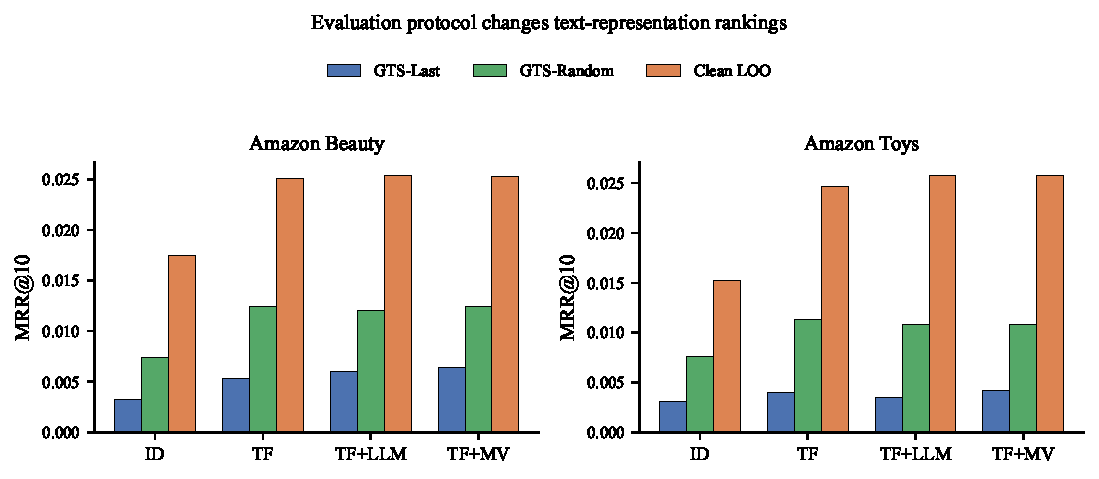
\includegraphics[width=\linewidth]{figures/fig_protocol_contrast_v2.pdf}
\caption{%
Protocol contrast on Beauty and Toys.
GTS-Last/Random: warm MRR@10 (3 training seeds; Random further averaged over 3 target-sampling seeds); LOO is per-user leave-one-out, shown for contrast only.
Bar heights are \emph{point estimates}; gaps within one seed-level std use $\approx$.
Per-row orderings are in Table~\ref{tab:protocol}.%
}
\label{fig:protocol}
\end{figure}

\begin{table}[t]
\centering
\caption{%
GTS-Last warm NDCG@10 and Hit@10 (3-seed mean$\pm$std).
\textbf{Bold}: highest value in the row (same rule as Table~\ref{tab:protocol}).
Among the \base-based variants, NDCG agrees with MRR.
UniSRec is strongest on Hit@10 (all three datasets) and on Toys and Grocery NDCG.
}
\label{tab:ndcg_hit}
\small
\setlength{\tabcolsep}{2.5pt}
\begin{tabular}{@{}llccccc@{}}
\toprule
Dataset & Metric & ID & TF & TF+LLM & TF+MV & UniSRec \\
\midrule
\multirow{2}{*}{Beauty}
 & NDCG & .0047\tiny{$\pm$.0007} & .0074\tiny{$\pm$.0006} & .0080\tiny{$\pm$.0009} & \textbf{.0087}\tiny{$\pm$.0003} & .0081\tiny{$\pm$.0003} \\
 & Hit  & .0098\tiny{$\pm$.0013} & .0146\tiny{$\pm$.0013} & .0146\tiny{$\pm$.0029} & .0167\tiny{$\pm$.0011} & \textbf{.0180}\tiny{$\pm$.0007} \\
\midrule
\multirow{2}{*}{Toys}
 & NDCG & .0046\tiny{$\pm$.0004} & .0056\tiny{$\pm$.0006} & .0046\tiny{$\pm$.0002} & .0057\tiny{$\pm$.0011} & \textbf{.0066}\tiny{$\pm$.0013} \\
 & Hit  & .0098\tiny{$\pm$.0013} & .0108\tiny{$\pm$.0011} & .0084\tiny{$\pm$.0004} & .0108\tiny{$\pm$.0027} & \textbf{.0154}\tiny{$\pm$.0030} \\
\midrule
\multirow{2}{*}{Grocery}
 & NDCG & .0048\tiny{$\pm$.0019} & .0062\tiny{$\pm$.0004} & .0063\tiny{$\pm$.0005} & .0077\tiny{$\pm$.0007} & \textbf{.0160}\tiny{$\pm$.0003} \\
 & Hit  & .0107\tiny{$\pm$.0041} & .0117\tiny{$\pm$.0009} & .0117\tiny{$\pm$.0007} & .0136\tiny{$\pm$.0007} & \textbf{.0338}\tiny{$\pm$.0007} \\
\bottomrule
\end{tabular}
\end{table}

\begin{table}[t]
\centering
\caption{%
Per-seed GTS-Last warm MRR@10 (seeds 42 / 2024 / 2026).
Variance is visible; \tfmv's lead is small and seed-dependent.%
}
\label{tab:perseed}
\small
\setlength{\tabcolsep}{3pt}
\begin{tabular}{@{}llccccc@{}}
\toprule
Dataset & Seed & ID & TF & TF+LLM & TF+MV & UniSRec \\
\midrule
\multirow{3}{*}{Beauty}
 & 42    & .0038 & .0049 & .00627 & \textbf{.00629} & .0050 \\
 & 2024  & .0032 & .0052 & .0055 & \textbf{.0066} & .0054 \\
 & 2026  & .0026 & .0057 & \textbf{.0063} & .0061 & .0051 \\
\midrule
\multirow{3}{*}{Toys}
 & 42    & .0033 & \textbf{.0045} & .0037 & .0035 & .0044 \\
 & 2024  & .0030 & .0038 & .0032 & .0042 & \textbf{.0045} \\
 & 2026  & .0029 & .0036 & .0036 & \textbf{.0048} & .0031 \\
\bottomrule
\end{tabular}
\end{table}

Table~\ref{tab:protocol} and Figure~\ref{fig:protocol} report the protocol contrast.
No text representation wins everywhere; instead, the relative ordering shifts with the target-selection protocol:

\begin{itemize}[leftmargin=*,itemsep=1pt]
\item \textbf{GTS-Last}: among the controlled \base-based variants, point estimates favor \tfmv on Beauty and Grocery ($.0064$ / $.0058$); on Toys TF+MV${}\approx{}$TF ($.0042$ / $.0040$), with seed-dependent winners (Table~\ref{tab:perseed}); the adapted UniSRec baseline is strongest on Grocery ($.0107$).
\item \textbf{GTS-Random} (3 target-sampling seeds): TF leads on Toys ($.0113$ vs.\ \tfmv $.0108$, within one std of \tfmv); Beauty is a 4-decimal tie (TF $.01239$, \tfmv $.01244$, both round to $.0124$); Grocery is a tie (TF $.0087$, \tfmv $.0089$).
\item \textbf{LOO}: absolute MRR is 4--7$\times$ higher than GTS-Last; ranking becomes \tfllm $\approx$ \tfmv $\approx$ TF.
\end{itemize}
Last vs.\ Random is a \emph{target-selection} effect on the same trained GTS checkpoints; LOO vs.\ GTS is a \emph{split/training-protocol} effect (different training data and models).

\paragraph{A plausible account of the LOO gap.}
The 4--7$\times$ higher absolute scores under LOO also change the relative ordering among text methods.
LOO permits temporal overlap: a user's training interactions include items from the same time period as the test target, so co-occurrence statistics that would not exist under a strict temporal cutoff remain available.
This overlap may disproportionately benefit representations capturing fine-grained semantic similarity (\tfllm and \tfmv), since overlapping items provide richer co-occurrence signal for semantic features than for lexical ones.
Under GTS, where training and evaluation interactions are separated by a global temporal cutoff, that LOO ranking is no longer visible and \tfidf becomes competitive.

\paragraph{Why do Last and Random disagree?}
Under GTS-Last, each user's single evaluation target is their \emph{chronologically last} test interaction; under GTS-Random, it is uniformly sampled from the test window.
A text representation that ``wins'' under one target mode can ``lose'' under another, even with identical model weights.
Last may over-represent recently popular or niche items while Random draws a broader mix; regardless of the cause, our claim is only that changing target selection on the same checkpoints changes the winner.
This is not an artifact of the two modes scoring slightly different warm cohorts: restricting both to their intersecting warm users preserves the pattern (Appendix~\ref{app:intersection}).

\paragraph{Implications.}
All text methods outperform ID-only under every protocol we evaluate ($+$13--100\% relative under GTS-Last); absolute scores are higher under Random.

\paragraph{UniSRec as external baseline.}
Under the same GTS-Last protocol, users with at least five training interactions, and warm-target filtering, UniSRec scores $0.0052$ (Beauty) and $0.0040$ (Toys), between ID and TF on Beauty and tied with TF on Toys, but it leads on Grocery ($0.0107$, nearly $2\times$ the next best).
Table~\ref{tab:ndcg_hit} shows that NDCG@10 largely agrees with MRR rankings under GTS-Last, while Hit@10 elevates UniSRec across all three datasets, so metric choice interacts with protocol.
We therefore treat MRR as the primary ranking metric and report NDCG/Hit for completeness.
UniSRec's apparent ranking is protocol-sensitive: GTS-All warm is $.0180$ / $.0139$ on Beauty / Toys, versus GTS-Last warm $.0052$ / $.0040$ on the same checkpoints (Appendix~\ref{app:unisrec}).
Target mode and candidate scope can each shift where an external baseline appears to rank.

%==============================================================================
\section{RQ2: Temporal Robustness}
\label{sec:rq2}
%==============================================================================

\begin{table}[t]
\centering
\caption{%
Main ($80\%$ cutoff) vs.\ Early ($60\%$ cutoff) on Beauty --- GTS-Last warm MRR@10 (3-seed mean$\pm$std).
Early: first 60\% train, next 10\% valid, next 10\% test (final 20\% unused).
Fusion and cutoff-fit embeddings matched to Main; hyperparameters frozen.
The Main row matches Table~\ref{tab:protocol}.
Point estimates: \tfmv{} on Main, \tfidf{} on Early (within one std of \tfmv).%
}
\label{tab:early}
\small
\begin{tabular}{@{}lccc@{}}
\toprule
Window & TF & TF+LLM & TF+MV \\
\midrule
Main      & .0053\tiny{$\pm$.0004} & .0060\tiny{$\pm$.0004} & \textbf{.0064}\tiny{$\pm$.0003} \\
Early60-EQ & \textbf{.0042}\tiny{$\pm$.0005} & .0037\tiny{$\pm$.0003} & .0039\tiny{$\pm$.0003} \\
\bottomrule
\end{tabular}
\end{table}

\begin{table}[t]
\centering
\caption{%
All-target catalog-level context (valid$\to$test, Main GTS), \emph{not} a direct explanation of warm-target MRR.
Unseen targets are absent from the train catalog and never enter the warm scores of Tables~\ref{tab:protocol} and~\ref{tab:early}.
Reported as associations with catalog shift, not causal claims.%
}
\label{tab:shift}
\small
\setlength{\tabcolsep}{4pt}
\begin{tabular}{@{}lccc@{}}
\toprule
Dataset & Unseen targets & Pop mean (V$\to$T) & Pop median (V$\to$T) \\
\midrule
Beauty  & 31.9\% & $112.8 \to 101.8$ & $21 \to 15$ \\
Toys    & 40.8\% & $144.7 \to 119.1$ & $18 \to 11$ \\
Grocery & 29.6\% & $87.3 \to 76.9$ & $16 \to 12$ \\
\bottomrule
\end{tabular}
\end{table}

\begin{table}[t]
\centering
\caption{%
All-target popularity-bucket composition (valid$\to$test, Main GTS; head $\ge$10, mid 3--9, low 1--2 train interactions).%
}
\label{tab:bucket}
\small
\setlength{\tabcolsep}{3.5pt}
\begin{tabular}{@{}llcccc@{}}
\toprule
Dataset & Split & Head & Mid & Low & Unseen \\
\midrule
\multirow{2}{*}{Beauty}
 & Valid & 63.1\% & 15.9\% & 9.7\% & 11.3\% \\
 & Test  & 56.6\% & 14.9\% & 10.7\% & 17.8\% \\
\midrule
\multirow{2}{*}{Toys}
 & Valid & 60.1\% & 16.3\% & 10.6\% & 13.0\% \\
 & Test  & 52.3\% & 15.5\% & 11.0\% & 21.3\% \\
\bottomrule
\end{tabular}
\end{table}

Table~\ref{tab:early} reports GTS-Last warm MRR@10 on Beauty for both windows under the same cutoff-fit protocol.
Absolute scores drop from Main to Early for every variant.
The within-window ranking is \emph{not} invariant: point estimates favor \tfmv on Main and \tfidf on Early ($.0042$ vs.\ \tfmv $.0039$ and \tfllm $.0037$, within one std of \tfmv).
All three remain within $0.001$ of each other.
The Main$\to$Early drop in Table~\ref{tab:early} is measured on warm targets only.
Tables~\ref{tab:shift}--\ref{tab:bucket} provide all-target \emph{catalog-level context} (unseen share, popularity) for the same global cutoffs; they are not a direct explanation of warm-MRR degradation, because unseen items never enter those scores.

\paragraph{TF-IDF robustness under shift.}
\tfidf exhibits the smallest Main-to-Early drop among the three text variants (Table~\ref{tab:early}); we treat this as an empirical robustness observation rather than evidence for a causal mechanism.

%==============================================================================
\section{RQ3: Why Limited Multi-View Gain}
\label{sec:rq3}
%==============================================================================

\begin{figure}[t]
\centering
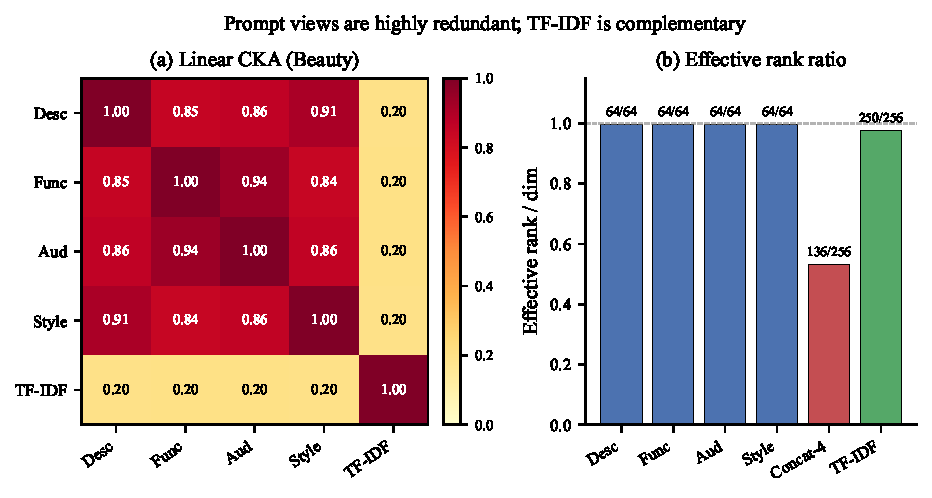
\includegraphics[width=\linewidth]{figures/fig_cka_heatmap.pdf}
\caption{%
Representation analysis on Beauty (3 random item subsamples of 3{,}000 each, mean$\pm$std).
\textbf{(a)}~Pairwise CKA: LLM views show high mutual similarity (0.82--0.94); TF--LLM CKA is low (0.18--0.20).
\textbf{(b)}~Effective rank: 4-view concat 136--141/256 (53--55\%) vs.\ TF-IDF 250/256 (98\%).%
}
\label{fig:cka}
\end{figure}

\begin{table}[t]
\centering
\caption{%
Inter-view CKA (3 subsamples of 3K items, mean$\pm$std).
LLM view pairs lie in $0.82$--$0.94$ except Toys Function--Style ($.818$); TF-IDF vs.\ any LLM view stays within 0.18--0.20.%
}
\label{tab:cka}
\small
\setlength{\tabcolsep}{4pt}
\begin{tabular}{@{}lcc@{}}
\toprule
View Pair & Beauty & Toys \\
\midrule
Description--Function  & $.846 \pm .001$ & $.834 \pm .001$ \\
Description--Audience  & $.860 \pm .001$ & $.856 \pm .002$ \\
Description--Style     & $.914 \pm .000$ & $.904 \pm .001$ \\
Function--Audience     & $.940 \pm .000$ & $.921 \pm .001$ \\
Function--Style        & $.843 \pm .001$ & $.818 \pm .002$ \\
Audience--Style        & $.859 \pm .001$ & $.838 \pm .002$ \\
\midrule
\emph{TF-IDF vs.\ LLM view (range)} & $.196$--$.201$ & $.184$--$.189$ \\
\bottomrule
\end{tabular}
\end{table}

\begin{table}[t]
\centering
\caption{%
Effective rank (Beauty/Toys, 3 subsamples).
4-view concat occupies only 53--55\% of its nominal dimensionality.%
}
\label{tab:effrank}
\small
\begin{tabular}{@{}lccc@{}}
\toprule
Representation & Dim & ER (Beauty) & ER (Toys) \\
\midrule
Single LLM view (avg) & 64 & 63.7 (99.5\%) & 63.6 (99.4\%) \\
4-view concat & 256 & 136.1 (\textbf{53.2\%}) & 141.2 (\textbf{55.2\%}) \\
TF-IDF (SVD) & 256 & 249.9 (97.6\%) & 251.4 (98.2\%) \\
\bottomrule
\end{tabular}
\end{table}

\begin{table}[t]
\centering
\caption{%
Leave-one-view-out (LOVO; zero-mask, 3-seed mean) under GTS-Last warm, matching Table~\ref{tab:protocol}.
$\Delta$: warm MRR@10 change vs.\ the full 4-view model.
Maximum $|\Delta|{=}0.00032$ (Style on Beauty).%
}
\label{tab:lovo}
\small
\setlength{\tabcolsep}{3.5pt}
\begin{tabular}{@{}lccccc@{}}
\toprule
Dataset & Full MRR & $-$Desc & $-$Func & $-$Aud & $-$Style \\
\midrule
Beauty & .00636 & $-$.00021 & $-$.00030 & $-$.00027 & $-$.00032 \\
Toys   & .00417 & $-$.00017 & $+$.00005 & $-$.00007 & $-$.00025 \\
\bottomrule
\end{tabular}
\end{table}

We address RQ3 with three complementary analyses, none of which is sufficient alone: CKA measures Gram-matrix similarity~\cite{kornblith2019cka}, effective rank measures dimensionality utilization, and LOVO measures downstream impact.

\paragraph{(1) High inter-view CKA.}
Table~\ref{tab:cka} and Figure~\ref{fig:cka}(a) show that LLM view pairs have CKA $0.82$--$0.94$ (Beauty $0.84$--$0.94$; Toys $0.82$--$0.92$, except Function--Style $.818$).
The four prompt views, generated from the same encoder applied to the same item text with different instructions, encode highly similar relational structures.
In contrast, TF-IDF vs.\ any LLM view yields CKA 0.196--0.201 (Beauty) and 0.184--0.189 (Toys)---a qualitatively different regime indicating substantial representational dissimilarity.

\paragraph{(2) Pairwise cosine vs.\ CKA.}
Mean pairwise cosine between prompt views is often moderate or near zero (e.g., Description--Function $\approx -0.01$ on Beauty), while Function--Audience reaches $\approx 0.42$.
This does \emph{not} contradict high CKA: cosine measures instance-level alignment of vectors, whereas CKA compares Gram-matrix geometry across the item set~\cite{kornblith2019cka}.
Views can have low average cosine yet still induce nearly isomorphic similarity structures, which is the regime we observe for prompt-based paraphrasing.
We therefore treat CKA as the primary similarity diagnostic and use cosine only as a complementary check, never as standalone proof of redundancy.

\paragraph{(3) Low effective rank of concatenated views.}
Table~\ref{tab:effrank} and Figure~\ref{fig:cka}(b) show that concatenating four 64-d views into 256 dimensions yields effective rank of only 136 (Beauty) and 141 (Toys), occupying 53--55\% of the available capacity.
Nearly half the nominal dimensions carry redundant structure.
TF-IDF at the same 256-d has effective rank $\ge$250 (97--98\%), utilizing almost all capacity.
Concatenating prompt views therefore expands the subspace far less than the dimension count suggests.

\paragraph{(4) Negligible LOVO impact.}
Table~\ref{tab:lovo} shows that zeroing any single view has minimal downstream effect under GTS-Last warm: maximum $|\Delta|{=}0.00032$ (${\approx}\,5\%$ of the full \tfmv score).
Full MRR matches Table~\ref{tab:protocol}'s \tfmv column.
Per-seed signs can flip, so we do not treat any prompt as uniquely necessary.

\paragraph{Where is redundancy already present?}
To disentangle prompt-induced from preprocessing-induced redundancy, we compare CKA at two stages: \emph{pre-whitening} (SVD-projected + centered, 64-d per view, without ZCA whitening) and \emph{post-whitening} (the final model-input embeddings).
On Beauty, mean pairwise CKA is $0.96\pm0.001$ pre-whitening and $0.88\pm0.001$ post-whitening; on Toys, $0.96\pm0.001$ and $0.87\pm0.001$ respectively.
CKA is \emph{already extremely high before whitening} (Table~\ref{tab:cka-prepost}): whitening \emph{reduces} mean inter-view CKA by 0.08 (Beauty) and 0.10 (Toys), and raises concatenated effective rank from 99/256 (39\%) to 136/256 (53\%) on Beauty and from 104/256 to 140/256 on Toys.

To trace redundancy further upstream, we compute inter-view CKA directly on the raw 3584-d Qwen hidden states \emph{before any SVD projection}.
Mean pairwise CKA at 3584-d is $0.961$ on Beauty and $0.963$ on Toys (3-trial random subsample of 3000 items, $\sigma < 0.002$).
Redundancy is therefore already present in the raw Qwen outputs before SVD or whitening under our prompt design, rather than an artifact of SVD truncation.
We cannot separate encoder geometry from the shared item text or from limited prompt divergence: even at this stage the four views yield near-isomorphic relational structures.
Whitening partially decorrelates the views but cannot remove this structural overlap.
A wider per-view projection is thus unlikely to remove the overlap (Table~\ref{tab:cka-prepost}).

\begin{table}[t]
\centering
\caption{%
Pre- vs.\ post-whitening audit (3 item-subsamples, mean).
CKA is already $\ge$0.94 before whitening; whitening lowers CKA and raises concat effective rank, so redundancy is not a whitening artifact.
Subsamples are drawn independently of Table~\ref{tab:effrank}, hence the $\pm 1$ difference in the Toys post-whitening rank.%
}
\label{tab:cka-prepost}
\small
\begin{tabular}{@{}llcc@{}}
\toprule
Dataset & Stage & Pairwise CKA & Concat ER/256 \\
\midrule
\multirow{2}{*}{Beauty}
 & Pre-whiten (SVD+center)  & 0.94--0.99 & 99 (39\%) \\
 & Post-whiten (TS fit)     & 0.84--0.94 & 136 (53\%) \\
\midrule
\multirow{2}{*}{Toys}
 & Pre-whiten (SVD+center)  & 0.94--0.98 & 104 (41\%) \\
 & Post-whiten (TS fit)     & 0.82--0.92 & 140 (55\%) \\
\bottomrule
\end{tabular}
\end{table}

\paragraph{Synthesis.}
The three diagnostics agree: prompt views encode overlapping semantics, which produces dimensionality collapse and negligible per-view contribution.
The observed geometry is consistent with insufficient view complementarity for views derived from a single source via semantic paraphrasing~\cite{xu2013multiview}.
The potential complementarity in our system lies between lexical \tfidf and semantic \llm views (CKA $0.18$--$0.20$).

%==============================================================================
\section{Discussion and Limitations}
\label{sec:discussion}
%==============================================================================

\paragraph{Why does TF-IDF alone match \tfmv?}
Under GTS-Random, \tfidf matches or exceeds the four-view variant on warm targets (Table~\ref{tab:protocol}).
First, \tfidf captures \emph{lexical diversity}: the vocabulary of product titles and descriptions spans tens of thousands of unique tokens, and SVD-projected TF-IDF retains nearly all available capacity (ER/dim $\approx$0.98; Table~\ref{tab:effrank}).
Second, the four LLM views share highly similar relational geometry (CKA $0.82$--$0.94$) because the same encoder processes the same item text with only minor instruction changes.
Concatenating them nominally quadruples dimensionality but only about doubles the effective rank ($64 \to 136$), so the concatenated views occupy about half of their nominal rank (Table~\ref{tab:effrank}).

\paragraph{LLM-only (no \tfidf base) ablation.}
Because \tfllm and \tfmv augment the \tfidf base, one may ask how much the LLM views achieve on their own.
We train a variant using only a single Qwen2.5-7B view with \emph{no} \tfidf base (same architecture, same two-phase pipeline).
Under the main protocol (GTS-Last, warm targets, users with $\ge 5$ training interactions, train-catalog candidates), this LLM-only variant scores $.0046\pm.0001$ on Beauty and $.0018\pm.0007$ on Toys---below the \tfllm column in Table~\ref{tab:protocol} ($.0060$ / $.0035$) and below ID-only on Toys.
The lexical base is therefore load-bearing, not a ``free init'': all of our text gains are gains of \tfidf-anchored pipelines.

\paragraph{Single-view hybrid: dropping three of the four views.}
To test whether the lexical--semantic dissimilarity identified in RQ3 (TF--LLM CKA $0.18$--$0.20$) is usable at ranking time, we train a hybrid that keeps the \tfidf base and a \emph{single} LLM view inside the multi-view architecture (per-view projection + concatena\-tion; no extra prompt views), under the same cutoff-fit protocol and training seeds as Table~\ref{tab:protocol}.
Under GTS-Last warm, the hybrid scores $.0070\pm.0006$ (Beauty) and $.0049\pm.0011$ (Toys), vs.\ \tfmv $.0064\pm.0003$ / $.0042\pm.0006$; under GTS-Random (3 target-sampling seeds) it scores $.0128\pm.0003$ and $.0114\pm.0008$, vs.\ \tfmv $.01244\pm.0002$ / $.0108\pm.0009$.
The hybrid thus matches or slightly exceeds the four-view model on both datasets under both target modes while using one prompt view instead of four, with margins within one seed-level std---\emph{no loss from dropping three views}, not a large additive gain.
Low TF--LLM CKA by itself licenses only \emph{geometric dissimilarity}; the hybrid provides the ranking-level evidence.

\paragraph{Implications.}
\begin{enumerate}[leftmargin=*,itemsep=2pt]
\item Report text-representation comparisons under GTS with explicit target mode.
\item Start with cutoff-fit \tfidf as a strong baseline.  Under GTS-Random it stays within one std of \tfmv on all three datasets and leads on Toys; under GTS-Last on the Main window it may trail \tfllm/\tfmv, but Table~\ref{tab:early} shows that an earlier cutoff can reverse that ranking on Beauty.  Given its negligible preprocessing cost relative to LLM inference, TF-IDF should be the first text baseline evaluated.
\item Diagnose redundancy (e.g., via CKA and effective rank) before adding more prompt views.
\item In our runs, a \tfidf + single-LLM-view hybrid matched or slightly exceeded \tfmv under both GTS-Last and GTS-Random.
\end{enumerate}

\paragraph{Limitations.}
\begin{itemize}[leftmargin=*,itemsep=1pt]
\item \textbf{Warm-target scope.}
Our models lack content-only zero-shot fallback; warm-target evaluation is thus the fairest comparison, but it excludes 30--38\% of eligible users' last test targets (and 30--41\% of all post-cutoff targets).
\item \textbf{Static metadata.}
We use fixed product titles/descriptions; temporally evolving text (e.g., reviews, trending tags) could change the TF/LLM balance.
\item \textbf{Amazon-only domain.}
All three datasets are Amazon subcategories.  Grocery is a same-platform replication, not a solution to domain diversity.
\item \textbf{GTS-Random reproducibility.}
Random is non-deterministic~\cite{gusak2025time}; the 0.001--0.003 cross-seed std in Section~\ref{sec:protocol} is measured on our checkpoints.
\item \textbf{Redundancy locus.}
Our audit spans raw 3584-d Qwen hidden states through 64-d post-whitening, showing redundancy already present before SVD/whitening (Section~\ref{sec:rq3}).  Only one LLM (Qwen2.5-7B) is tested; we cannot isolate encoder geometry from shared item text or prompt similarity.
\item \textbf{Successive protocol.}
\citet{gusak2025time} identify Successive---scoring every test interaction in chronological order---as the closest offline analogue of online next-item prediction, and treat Last/Random as cheaper proxies with high rank-correlation to it.
We report Last and Random; full Successive scoring at sampled-user scale remains future work.
\end{itemize}

\paragraph{Cost analysis.}
\begin{table}[t]
\centering
\caption{Recommendation-stage parameter count and online scoring cost (seed~42; \emph{offline text encoding excluded}).  \tfmv adds $<$1\% parameters.}
\label{tab:cost}
\small
\begin{tabular}{@{}lcc@{}}
\toprule
Model & Params (M) & ms/sample \\
\midrule
ID / TF / TF+LLM / TF+MV & 67.2 / 67.4 / 67.6 / 67.7 & 0.02 \\
UniSRec & 67.7 & 0.04 \\
\bottomrule
\multicolumn{3}{@{}l}{\footnotesize Beauty; Toys is $\sim$87M due to larger vocab (ranking identical).}
\end{tabular}
\end{table}

Table~\ref{tab:cost} shows that limited multi-view gains are not a recommendation-stage capacity issue: all variants have effectively the same parameter budget and online scoring cost.
The practical cost gap lies in \emph{offline text encoding}, which the table deliberately excludes: cutoff-fit \tfidf+SVD takes about a minute on CPU for the Beauty catalog (259K items, measured), whereas each Qwen2.5-7B view requires a one-time GPU inference pass over the catalog, and multi-view multiplies that pass by the number of prompts.
Feature-side cost, not model-side cost, is where \tfidf, \tfllm, and \tfmv differ.

%==============================================================================
\section{Conclusion}
\label{sec:conclusion}
%==============================================================================

We conducted a leakage-aware controlled study of text representations for sequential recommendation, structured as an empirical investigation rather than a model-proposal paper.

\begin{enumerate}[leftmargin=*,itemsep=1pt]
\item \textbf{Protocol matters.}
The relative ordering of \tfidf, \tfllm, and \tfmv depends on the GTS target mode.
Text features consistently outperform ID-only, but which text is best requires specifying the evaluation protocol.
Among the \base-based variants under GTS-Last, point estimates favor \tfmv on Beauty and Grocery, while Toys is TF+MV${}\approx{}$TF (the adapted UniSRec baseline is strongest on Grocery); under GTS-Random, \tfidf catches up and overtakes it on Toys, with no gap exceeding one std. This shift is driven entirely by target selection, not by model changes.
\item \textbf{No text variant is consistently dominant.}
Under a matched-protocol equal-horizon Early window on Beauty ($60\%$ cutoff; the same $10\%$ valid/\hspace{0pt}test spans as Main, final $20\%$ unused), absolute MRR drops and the Main ranking is not preserved (\tfidf leads narrowly), yet text variants remain within 0.001 of each other.
\item \textbf{Multi-view gains are limited by inter-view redundancy.}
CKA, effective rank, and LOVO jointly show that prompt views encode overlapping semantics; potential complementarity lies between lexical and semantic features (CKA $0.18$--$0.20$), not between different prompt instructions applied to the same encoder.
Consistently, a hybrid that keeps the \tfidf base and a single LLM view matches or slightly exceeds \tfmv under both GTS-Last and GTS-Random (Section~\ref{sec:discussion}).
\end{enumerate}

The practical default under leakage-aware evaluation is: report GTS-Last (and Random as a check), keep cutoff-fit \tfidf as a mandatory baseline, and treat multi-view LLM features as a hypothesis to be tested---not a free upgrade.

\paragraph{Future directions.}
Five questions remain open.
(1)~\textbf{Richer lexical--semantic fusion.}  Whether more sophisticated fusion (e.g., gating, cross-attention) can turn the lexical--semantic pair into larger, significant gains remains open.
(2)~\textbf{Cross-architecture redundancy audit.}  Our raw 3584-d audit finds this redundancy already in Qwen2.5-7B outputs under our prompt design.  Testing whether the same inter-view collapse holds for decoder-only vs.\ encoder-only LLMs (e.g., Mistral, BERT-\hspace{0pt}large) would clarify whether this is a general transformer property or specific to the Qwen family.
(3)~\textbf{GTS-Successive evaluation} at sampled-user scale, to validate Last/Random as proxies for online next-item prediction~\cite{gusak2025time}.
(4)~\textbf{Non-Amazon domains} with reliable timestamps, to test whether protocol sensitivity generalizes beyond product catalogs.
(5)~\textbf{Instruction-diverse prompts} that enforce semantic divergence (e.g., attribute extraction vs.\ sentiment summarization) to test whether complementarity can be engineered at the prompt level.

\section*{Ethical Considerations}
This work uses public Amazon review datasets with no personally identifiable attributes beyond standard user/item IDs.
Potential concerns include reinforcing popularity bias under temporal shift and inheriting biases from LLM-generated text features.
We report warm-target stratified diagnostics.
No human subjects were involved.

\begin{acks}
Anonymous for review.
\end{acks}

%==============================================================================
\appendix
\renewcommand{\arraystretch}{0.88}
\setlength{\abovecaptionskip}{4pt}
\setlength{\belowcaptionskip}{2pt}
%==============================================================================

\section{GTS-All Results}
\label{app:gts-all}

Main tables use GTS-Last (one last target per user).
GTS-All evaluates all post-cutoff targets (Beauty: 4{,}520 users $\to$ 12{,}001 samples, avg 2.65/user; Toys: 4{,}873 users $\to$ 13{,}186, avg 2.71/user).

\begin{table}[H]
\centering
\caption{GTS-All warm MRR@10 (3-seed mean; cutoff-fit checkpoints for all columns).
Beauty TF/\tfmv to 5 decimals because both round to $.0241$.
\textbf{Bold}: row max (same rule as Table~\ref{tab:protocol}).}
\label{tab:gts-all}
\small
\begin{tabular}{@{}lccccc@{}}
\toprule
Dataset & ID & TF & TF+LLM & TF+MV & UniSRec \\
\midrule
Beauty & .0156 & .02411 & .0237 & \textbf{.02413} & .0180 \\
Toys   & .0118 & \textbf{.0191} & .0180 & .0184 & .0139 \\
\bottomrule
\end{tabular}
\end{table}

Under GTS-All, TF leads \tfmv on Toys and trails it by $.00002$ on Beauty, closer to the GTS-Random picture than to GTS-Last, where \tfmv leads narrowly among the \base-based variants.
All has the lowest rank-correlation with Successive and introduces task mismatch~\cite{gusak2025time}.

\section{Grocery Per-Seed Breakdown}
\label{app:grocery}

Grocery replicates the Beauty/Toys pattern under the same search budget: among the \base-based variants, \tfmv leads narrowly on Last, and TF and \tfmv stay within one std of each other on Random.

\begin{table}[H]
\centering
\caption{Grocery warm MRR@10 per training seed under GTS-Last and GTS-Random (Random averaged over target-sampling seeds $\{42,123,456\}$).
\textbf{Bold}: row max among ID/TF/TF+LLM/TF+MV.}
\label{tab:grocery-perseed}
\small
\setlength{\tabcolsep}{3pt}
\begin{tabular}{@{}llcccc@{}}
\toprule
Protocol & Seed & ID & TF & TF+LLM & TF+MV \\
\midrule
\multirow{3}{*}{GTS-Last}
 & 42    & .0027 & .0038 & .0049 & \textbf{.0052} \\
 & 2024  & .0019 & .0049 & .0050 & \textbf{.0058} \\
 & 2026  & .0043 & .0050 & .0041 & \textbf{.0065} \\
\midrule
\multirow{3}{*}{GTS-Rand}
 & 42    & .0044 & .0075 & .0073 & \textbf{.0088} \\
 & 2024  & .0041 & \textbf{.0095} & .0080 & .0082 \\
 & 2026  & .0063 & .0091 & .0075 & \textbf{.0097} \\
\bottomrule
\end{tabular}
\end{table}

\section{GTS-Random Target-Sampling Seeds}
\label{app:random-seeds}

Main-table GTS-Random numbers average three target-sampling seeds $\{42,123,456\}$ on the same checkpoints (no retraining).
Table~\ref{tab:random-seeds} reports each seed after averaging the three training seeds.
Cross-seed std of warm MRR@10 is typically 0.001--0.003; seed~456 is systematically lower, which is why a single Random seed would overstate TF's Beauty lead (0.0138 vs.\ 3-seed 0.01239).

\begin{table}[H]
\centering
\caption{GTS-Random warm MRR@10 by target-sampling seed (mean over training seeds 42/2024/2026).
\textbf{Bold}: row max.}
\label{tab:random-seeds}
\small
\setlength{\tabcolsep}{3pt}
\begin{tabular}{@{}llccccc@{}}
\toprule
Dataset & Target seed & ID & TF & TF+LLM & TF+MV & UniSRec \\
\midrule
\multirow{3}{*}{Beauty}
 & 42    & .0081 & \textbf{.0138} & .0133 & .0134 & .0098 \\
 & 123   & .0080 & .0134 & .0128 & \textbf{.0141} & .0103 \\
 & 456   & .0063 & \textbf{.0101} & .0099 & .0098 & .0087 \\
\midrule
\multirow{3}{*}{Toys}
 & 42    & .0096 & \textbf{.0146} & .0140 & .0141 & .0103 \\
 & 123   & .0066 & \textbf{.0091} & .0089 & .0085 & .0078 \\
 & 456   & .0065 & \textbf{.0101} & .0095 & .0098 & .0075 \\
\bottomrule
\end{tabular}
\end{table}

\section{Last vs.\ Random on Intersecting Users}
\label{app:intersection}

Last and Random score the same eligible users, but the warm filter applies to the \emph{selected} target, so the two warm sub-cohorts do not coincide exactly (Section~\ref{sec:protocol}).
We re-score both modes on the \emph{intersection} of their warm cohorts---users whose Last target \emph{and} whose Random target both lie in the train catalog---using the same checkpoints and a single forward pass per checkpoint, so that per-user ranks are identical to those behind the main tables.
The intersection retains 2{,}846--2{,}858 users on Beauty (63\% of eligible), 2{,}651--2{,}686 on Toys (54--55\%), and 2{,}671--2{,}678 on Grocery (64\%), varying only with the Random target-sampling seed.

\begin{table}[H]
\centering
\caption{Warm MRR@10 on intersecting users (warm under both Last and Random) vs.\ the full warm cohorts used in the main tables. Mean$\pm$std over 3 training seeds; Random additionally averages target-sampling seeds $\{42,123,456\}$. \textbf{Bold}: highest among ID/\tfidf/\tfllm/\tfmv in that column (same rule as Table~\ref{tab:protocol}; UniSRec not in this table).}
\label{tab:intersection}
\small
\setlength{\tabcolsep}{3pt}
\begin{tabular}{@{}llcccc@{}}
\toprule
& & \multicolumn{2}{c}{Last} & \multicolumn{2}{c}{Random} \\
\cmidrule(lr){3-4}\cmidrule(lr){5-6}
Dataset & Variant & Intersect. & Full warm & Intersect. & Full warm \\
\midrule
\multirow{4}{*}{Beauty}
 & ID     & .0033$\pm$.0007 & .0032$\pm$.0006 & .0066$\pm$.0005 & .0074$\pm$.0005 \\
 & \tfidf & .0054$\pm$.0004 & .0053$\pm$.0004 & .0110$\pm$.0003 & \textbf{.0124}$\pm$.0002 \\
 & \tfllm & .0063$\pm$.0005 & .0060$\pm$.0004 & .0107$\pm$.0003 & .0120$\pm$.0002 \\
 & \tfmv  & \textbf{.0065}$\pm$.0004 & \textbf{.0064}$\pm$.0003 & \textbf{.0113}$\pm$.0002 & \textbf{.0124}$\pm$.0002 \\
\midrule
\multirow{4}{*}{Toys}
 & ID     & .0032$\pm$.0002 & .0031$\pm$.0002 & .0073$\pm$.0001 & .0076$\pm$.0002 \\
 & \tfidf & .0039$\pm$.0006 & .0040$\pm$.0005 & \textbf{.0110}$\pm$.0004 & \textbf{.0113}$\pm$.0004 \\
 & \tfllm & .0035$\pm$.0002 & .0035$\pm$.0002 & .0106$\pm$.0007 & .0108$\pm$.0007 \\
 & \tfmv  & \textbf{.0040}$\pm$.0005 & \textbf{.0042}$\pm$.0006 & .0105$\pm$.0009 & .0108$\pm$.0009 \\
\midrule
\multirow{4}{*}{Grocery}
 & ID     & .0031$\pm$.0012 & .0030$\pm$.0012 & .0047$\pm$.0012 & .0050$\pm$.0012 \\
 & \tfidf & .0049$\pm$.0007 & .0046$\pm$.0006 & .0083$\pm$.0012 & .0087$\pm$.0011 \\
 & \tfllm & .0050$\pm$.0005 & .0047$\pm$.0005 & .0071$\pm$.0002 & .0076$\pm$.0004 \\
 & \tfmv  & \textbf{.0063}$\pm$.0006 & \textbf{.0058}$\pm$.0007 & \textbf{.0087}$\pm$.0009 & \textbf{.0089}$\pm$.0008 \\
\bottomrule
\end{tabular}
\end{table}

Table~\ref{tab:intersection} reports warm MRR@10 on the intersection alongside the full warm cohorts of Table~\ref{tab:protocol}.
Two observations hold in all six dataset$\times$mode blocks.
First, restricting to the intersection changes absolute scores by at most $.0014$ (largest on Beauty Random, where dropping the Last-only warm users lowers TF from $.0124$ to $.0110$) and does not change which of \tfidf and \tfmv leads.
Second, the Last$\to$Random shifts we rely on survive on the identical user set: point estimates favor \tfmv under Last on Beauty and Grocery, with Toys TF+MV${}\approx{}$TF, whereas under Random \tfidf closes to within one std on Beauty ($.0110$ vs.\ $.0113$) and Grocery ($.0083$ vs.\ $.0087$) and overtakes \tfmv on Toys ($.0110$ vs.\ $.0105$).
Random remains easier than Last for every variant.

\section{UniSRec Detailed Results}
\label{app:unisrec}

UniSRec~\cite{hou2022unisrec} is protocol-sensitive even under the shared filter (users with at least 5 training interactions; same cutoff-fit checkpoints):

\begin{table}[H]
\centering
\caption{UniSRec warm MRR@10 under the shared filter (3-seed mean$\pm$std).}
\label{tab:unisrec-app}
\small
\begin{tabular}{@{}lccc@{}}
\toprule
Dataset & GTS-All & GTS-Last & GTS-Random$^\dagger$ \\
\midrule
Beauty & .0180$\pm$.0001 & .0052$\pm$.0002 & .0096$\pm$.0001 \\
Toys   & .0139$\pm$.0003 & .0040$\pm$.0008 & .0085$\pm$.0003 \\
\bottomrule
\end{tabular}
\end{table}

\noindent$^\dagger$GTS-Random averaged over target-sampling seeds $\{42,123,456\}$ (same protocol as Table~\ref{tab:protocol}).
All three columns are warm-target MRR@10 on the same cutoff-fit checkpoints.

\balance
\bibliographystyle{ACM-Reference-Format}
\begingroup
\raggedbottom
\interlinepenalty=10000
\bibliography{refs}
\endgroup

\end{document}
